\documentclass{article}

\usepackage[
    mocha,
    pagecolor=true,
    textcolor=true
]{catppuccinpalette}
\usepackage[
    backend=biber,
    style=alphabetic,
    sorting=ynt
]{biblatex}
\usepackage{mdframed}
\usepackage{letltxmacro}
\usepackage{xcolor}
\usepackage{enumitem}
\usepackage[fixed]{fontawesome5}
\usepackage{titlesec}
\usepackage{abstract}
\usepackage{hyperref}
\usepackage[nottoc,numbib]{tocbibind}
\usepackage{tikz}
\usepackage{pgfplots}
\usepackage{caption}
\usepackage{multicol}
\usepackage{amsmath}

% Pgfplots 
\pgfplotsset{compat=1.18}

% Catppuccin mocha colors
\definecolor{rosewater}{HTML}{f5e0dc}   % Rosewater
\definecolor{flamingo}{HTML}{f2cdcd}    % Flamingo
\definecolor{pink}{HTML}{f5c2e7}        % Pink
\definecolor{mauve}{HTML}{cba6f7}       % Mauve
\definecolor{red}{HTML}{f38ba8}         % Red
\definecolor{maroon}{HTML}{eba0ac}      % Maroon
\definecolor{peach}{HTML}{fab387}       % Peach
\definecolor{yellow}{HTML}{f9e2af}      % Yellow
\definecolor{green}{HTML}{a6e3a1}       % Green
\definecolor{teal}{HTML}{94e2d5}        % Teal
\definecolor{sky}{HTML}{89dceb}         % Sky
\definecolor{sapphire}{HTML}{74c7ec}    % Sapphire
\definecolor{blue}{HTML}{89b4fa}        % Blue
\definecolor{lavender}{HTML}{b4befe}    % Lavender
\definecolor{text}{HTML}{cdd6f4}        % Text
\definecolor{subtext1}{HTML}{bac2de}    % Subtext 1
\definecolor{subtext0}{HTML}{a6adc8}    % Subtext 0
\definecolor{overlay2}{HTML}{9399b2}    % Overlay 2
\definecolor{overlay1}{HTML}{7f849c}    % Overlay 1
\definecolor{overlay0}{HTML}{6c7086}    % Overlay 0
\definecolor{surface2}{HTML}{585b70}    % Surface 2
\definecolor{surface1}{HTML}{45475a}    % Surface 1
\definecolor{surface0}{HTML}{313244}    % Surface 0
\definecolor{base}{HTML}{1e1e2e}        % Base
\definecolor{mantle}{HTML}{181825}      % Mantle
\definecolor{crust}{HTML}{11111b}       % Crust

% HREF
\hypersetup{
    colorlinks=true,
    linkcolor=peach,
    filecolor=yellow,
    urlcolor=sapphire
}

\urlstyle{same}

% Formatting
\titleformat{\section}
    {\normalfont\Large\bfseries\color{maroon}}
    {\thesection}{1em}{}

\titleformat{\subsection}
    {\normalfont\large\bfseries\color{peach}}
    {\thesubsection}{1em}{}

\titleformat{\subsubsection}
    {\normalfont\normalsize\bfseries\color{yellow}}
    {\thesubsubsection}{1em}{}

\renewcommand{\abstractname}{\color{red}\normalfont\normalsize\bfseries Abstract}

\setlist[enumerate,1]{label=\color{peach}\arabic*., font=\bfseries}
\setlist[enumerate,2]{label=\color{yellow}(\alph*), font=\bfseries}
\setlist[enumerate,3]{label=\color{green}\roman*., font=\bfseries}
\setlist[enumerate,4]{label=\color{teal}\Alph*., font=\bfseries}

\LetLtxMacro{\oldtextbf}{\textbf}
\renewcommand{\textbf}[1]{\oldtextbf{\color{mauve}#1}}
\LetLtxMacro{\oldtextit}{\textit}
\renewcommand{\textit}[1]{\oldtextit{\color{flamingo}#1}}

\everymath{\color{pink}}
\everydisplay{\color{pink}}

% Tikz Axis
\pgfplotsset{
    custom/.style={
        enlargelimits = true,
        thick,
        font = \small,
        axis line style = {rosewater},
        tick style = {rosewater},
        label style = {color = rosewater},
        xticklabel style = {color = rosewater},
        yticklabel style = {color = rosewater},
        legend pos = north east,
        legend style = {
            font=\small,
            draw=rosewater,
            fill=mantle
        }
    }
}

% Callouts
\mdfdefinestyle{calloutbase}{
  topline=false, rightline=false, bottomline=false,
  linewidth=2pt,
  innerleftmargin=10pt,
  innerrightmargin=10pt,
  innertopmargin=6pt,
  innerbottommargin=6pt,
  backgroundcolor=mantle,
  font=\color{subtext1},
}

\newmdenv[style=calloutbase, linecolor=sapphire]{cnote-base}
\newenvironment{cnote}[1][Note]{%
  \begin{cnote-base}%
  {\color{sapphire}\bfseries\faInfoCircle\hspace{0.5em}#1}\par\vspace{4pt}%
}{%
  \end{cnote-base}%
}

\newmdenv[style=calloutbase, linecolor=green]{ctip-base}
\newenvironment{ctip}[1][Tip]{%
  \begin{ctip-base}%
  {\color{green}\bfseries\faLightbulb\hspace{0.5em}#1}\par\vspace{4pt}%
}{%
  \end{ctip-base}%
}

\newmdenv[style=calloutbase, linecolor=peach]{cwarning-base}
\newenvironment{cwarning}[1][Warning]{%
  \begin{cwarning-base}%
  {\color{peach}\bfseries\faExclamationTriangle\hspace{0.5em}#1}\par\vspace{4pt}%
}{%
  \end{cwarning-base}%
}

\newmdenv[style=calloutbase, linecolor=overlay2]{cinfo-base}
\newenvironment{cinfo}[1][Further Information]{%
  \begin{cinfo-base}%
  {\color{overlay2}\bfseries\faBookOpen\hspace{0.5em}#1}\par\vspace{4pt}%
}{%
  \end{cinfo-base}%
}

% Citation file
\addbibresource{citations.bib}

\title{Audio Synthesizer}
\author{Pászti Tibor Miklós}

\begin{document}

\maketitle

\begin{abstract}
    The main goal for this paper is to describe the process of synthesizing
    music from a 
    \href{https://midi.org/}{MIDI}
    file, meaning that I read the given tracks and thus notes
    of the song beign supplied to the program and synthesize the audio based 
    on what oscillators and effects are present. The end product will be a 
    \href{https://en.wikipedia.org/wiki/Pulse-code_modulation}{PCM}
    file that could be converted to any other audio format needed.

    In this paper I will be talking about how to synthesize sound, alter 
    it with effects, how to build these effects and how to visualize the 
    synthesized audio in many forms.

    The examples in this paper will be shown in the c programing language
    and for the visual representation I will be using the 
    \href{https://wiki.libsdl.org/SDL3/FrontPage}{SDL3}
    library.

    Although I will be talking about some basic concepts I won't be 
    writing about these concept in an educational manner. I will be 
    citing the relevant sections of my sources that I will be using
    so for further or more indepth information I recommend reading
    the sources I will be using relating to audio synthesis.
    All the sources will be shown at the bibliography section of 
    the paper and they will also be cited at the relevant sections.
\end{abstract}

\tableofcontents
\pagebreak

\section{Basic Workings:}
In the most basic sense my synthesizer will go through the following steps:

\begin{enumerate}
    \item Read the MIDI file and store it in a fitting structure.
    \item Go through each track and it's notes and calculate the note's 
        amplitude at a given phase for the selected wavetable.
    \item If more than one note is active, then get the avarage of the amplitudes.
    \item Write every amplitude into a PCM audio file for playback.
    \item Play the audio with the SDL3 library's mixer.
\end{enumerate}

This describes a very basic synthesizer program, which I will
use to explain the core workings of a synthesizer, mainly speaking
about the second and third points talking about the calculating of
the amplitudes and how to combine these amplitudes.

\subsection{Waveforms and Their Representation:}
A waveform is any series of values with a repeating pattern. One occurance 
of this pattern is called a \textit{cycle} and the length of this cycle is the 
\textit{wavelength} or \textit{period}. 
As the period increases, the frequency of cycles per second decreases and the 
sound becomes "lower".

\begin{cnote}
    Frequency (\textbf{Hz}) states the number of cycles per second.
\end{cnote}

\subsubsection{Time-domain Representation:}
First I would like to state what exactly does it mean when
a wave goes above or below zero.

The sound people hear is actually the air pressure changing
over a period of time, so when a speaker is "moving" it is 
actually just changing the air pressure according to the analog 
signal beign supplied to it.

The \textbf{time-domain representation} is just a graph of air pressure 
over time.

To create an audible sound the frequency needs to be in the 
range of 20 Hz to 20 KHz. Any higher or lower and the 
human ear can't process it.

\newpage

\begin{cnote}
    The figures will be using a sample size of 4096
    because this will be the size of a waveform table as stated 
    in the future sections.
\end{cnote}

\begin{cwarning}[TODO]
    HREF TO THE RELEVANT SECTION.
\end{cwarning}

\begin{multicols}{2}
\begin{center}
        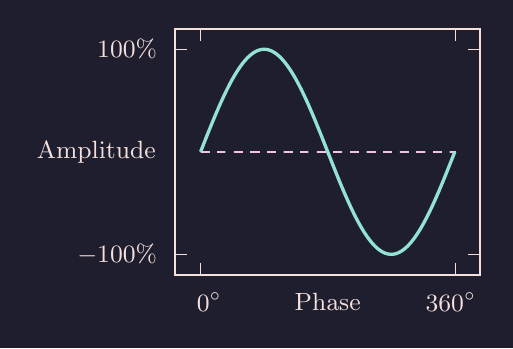
\begin{tikzpicture}
            \begin{axis}[
                custom,
                xlabel=Phase,
                ylabel=Amplitude,
                xlabel style = {anchor=south},
                ylabel style = {rotate=270, at={(axis cs:-4.3,0)}, anchor=west},
                domain=0:2*pi,
                ymin=-1, ymax=1,
                xtick = {0, 2*pi},
                xticklabels = {$0^{\circ}$, $360^{\circ}$},
                xticklabel style = {anchor=north east, xshift=4mm, yshift=-1mm},
                ytick = {-1, 1},
                yticklabels = {$-100\%$, $100\%$},
                yticklabel style = {anchor=east, xshift=-1mm}, 
                width=0.45*\textwidth,
                samples=4096
            ]
                \addplot[color=pink, dashed, forget plot]{0};
                \addplot[color=teal, very thick]{sin(deg(x))};
            \end{axis}
        \end{tikzpicture}
        \captionof{figure}{Sine Time-domain Representation}
    \end{center}

    \begin{center}
        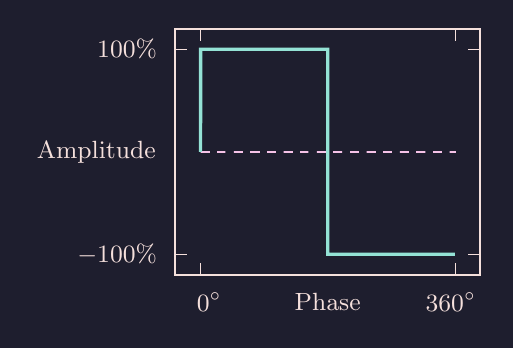
\begin{tikzpicture}
            \begin{axis}[
                custom,
                xlabel=Phase,
                ylabel=Amplitude,
                xlabel style = {anchor=south},
                ylabel style = {rotate=270, at={(axis cs:-4.3,0)}, anchor=west},
                domain=0:2*pi,
                ymin=-1, ymax=1,
                xtick = {0, 2*pi},
                xticklabels = {$0^{\circ}$, $360^{\circ}$},
                xticklabel style = {anchor=north east, xshift=4mm, yshift=-1mm},
                ytick = {-1, 1},
                yticklabels = {$-100\%$, $100\%$},
                yticklabel style = {anchor=east, xshift=-1mm}, 
                width=0.45*\textwidth,
                samples=4096
            ]
                \addplot[color=pink, dashed, forget plot]{0};
                \addplot[color=teal, very thick]{sign(sin(deg(x)))};
            \end{axis}
        \end{tikzpicture}
        \captionof{figure}{Square Time-domain Representation}
    \end{center}
\end{multicols}

When the amplitude is negative the air pressure is decreasing
and the same applies in the opposite manner. In the purest sense
the amplitude of a sound is describing the changes in air pressure.

\begin{cnote}
    As the topic moves to more abstract concepts the meaning of 
    amplitude will change to the volume level of a sound as a 
    range from 0 to 1.
\end{cnote}

\subsubsection{Frequency-domain Representation:}
Besides the \textit{fundamental frequency} beign supplied to the oscillator,
depending on the waveform there may be other \textit{overtones} or 
\textit{harmonics} present. 

For example the sine wave is said to be pure for one reason because
it has no overtones other than the fundamental frequency.
The \textbf{frequency-domain representation} exists to show these
overtones.

\newpage

\begin{multicols}{2}
    % --- Left Column: Sine Wave Frequency Domain ---
    \begin{center}
        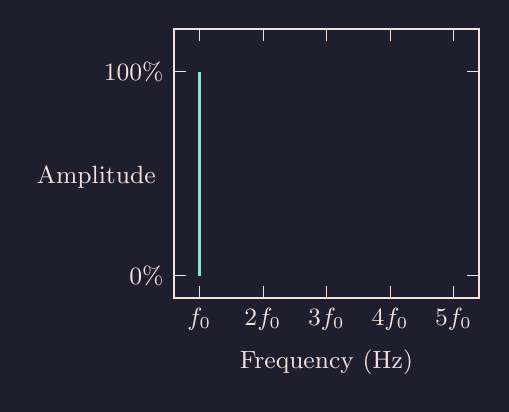
\begin{tikzpicture}
            \begin{axis}[
                custom,
                xlabel = {Frequency (Hz)},
                ylabel = {Amplitude},
                ylabel style = {rotate=270, at={(axis description cs:0, 0.45)}, anchor=east, xshift=-1mm},
                domain = 10:50,
                xmin = 10, xmax = 50,
                ymin = 0, ymax = 1.1,
                xtick = {10, 20, 30, 40, 50},
                xticklabels = {$f_0$, $2f_0$, $3f_0$, $4f_0$, $5f_0$},
                ytick = {0, 1},
                yticklabels = {$0\%$, $100\%$},
                width = 0.45\textwidth,
                height = 5cm
            ]
                % Pure Sine Wave Spectrum: Single peak at fundamental frequency (10 Hz)
                \addplot+[ycomb, color=teal, very thick, mark=none] coordinates {
                    (10, 1.0)
                };
            \end{axis}
        \end{tikzpicture}
        \captionof{figure}{Sine Frequency-domain Representation}
    \end{center}

    % --- Right Column: Square Wave Frequency Domain ---
    \begin{center}
        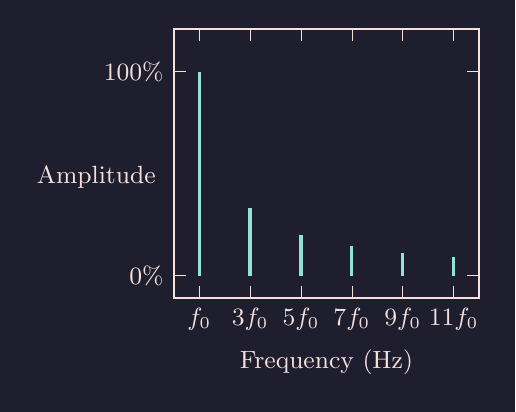
\begin{tikzpicture}
            % Programmatically calculate odd harmonics (1/n amplitude scaling)
            \edef\squarewavecoords{}
            \foreach \n in {1,3,5,7,9,11} {
                \pgfmathparse{1/\n}
                \xdef\squarewavecoords{\squarewavecoords (\n*10, \pgfmathresult)}
            }

            \begin{axis}[
                custom,
                xlabel = {Frequency (Hz)},
                ylabel = {Amplitude},
                ylabel style = {rotate=270, at={(axis description cs:0, 0.45)}, anchor=east, xshift=-1mm},
                domain = 10:110,
                xmin = 10, xmax = 110,
                ymin = 0, ymax = 1.1,
                xtick = {10, 30, 50, 70, 90, 110},
                xticklabels = {$f_0$, $3f_0$, $5f_0$, $7f_0$, $9f_0$, $11f_0$},
                ytick = {0, 1},
                yticklabels = {$0\%$, $100\%$},
                width = 0.45\textwidth,
                height = 5cm
            ]
                % Plot dynamically calculated odd harmonics
                \addplot+[ycomb, color=teal, very thick, mark=none] coordinates \squarewavecoords;
            \end{axis}
        \end{tikzpicture}
        \captionof{figure}{Square Frequency-domain Representation}
        \label{fig:square_freq}
    \end{center}
\end{multicols}

The frequency-domain representation is achieved by using the 
fourier transform on the given audio which will split it into 
a sum of sine waves with different amplitudes. This can be seen as
illustrated in Figure~\ref{fig:square_freq}.

\begin{cnote}
    The square waveforms frequency-domain representation is not 
    in it's full display to save space.
\end{cnote}

\begin{cinfo}
    For further information read the following source material \cite[pp.~14--18]{curtis}.
\end{cinfo}

\subsection{Waveform Table:}
As the number of notes and tracks grows so will the need 
for computational power and what does every note has to do?

Calculate a given number of trigonometric functions or even generate 
a bunch of random numbers if talking about a white noise sound.
To get around this I will be using a waveform table, meaning that
I will be storing the values of a given waveform in a table with a 
sample size of 4096.

This way I will be able to just index the current value of a sine 
function for example. This approach also lets the user draw their own
waveform tables afterwhich I can store it in a file and read it 
if the user wants to play that custom waveform.

$$ 
phase\_index = \text{mod}_L(previous\_phase + increment)
$$ 
$$
output = amplitude * wavetable[phase\_index]
$$

\begin{cnote}
    The mod operation is needed to not overindex the waveform table.
\end{cnote}

\subsection{Phase:}
The phase is what tells the oscillator how far along the waveform 
is in the time-domain representation and so I will have to increment
the phase for each note independently.

As seen in the previous section I will be using the phase to 
index the waveform table but first the increment needs to calculated
in the following way:

$$ 
increment = \frac{L * frequency}{samplingFrequency}
$$

\begin{cnote}
    With the table size beign a constant 4096 and the sampling frequency 
    or samplerate beign a constant 44.1KHz, this is not that big of a deal.
\end{cnote}

Due to understandable reasons this won't be a complete match 
to an actually calculated waveform and so slight ditrostions may 
occur. This is called \textit{table-lookup noise}.

As of now I hope this won't be too audible and I can 
ignore this slight problem.

\nocite{*}
\addcontentsline{toc}{section}{Bibliography}
\printbibliography[title=Bibliography] 

\end{document}
